%% tags: [aggregate analysis, depth first search]
%% source: 2023-sp-redemption_midterm_02
\begin{prob}

    Consider the code shown below. It shows DFS as seen in lecture, with one
    modification: a \mintinline{python}{print} statement in the for-loop.


    \begin{minted}[autogobble]{python}
        def dfs(graph, u, status=None):
            """Start a DFS at `u`."""
            # initialize status if it was not passed
            if status is None:
                status = {node: 'undiscovered' for node in graph.nodes}

            status[u] = 'pending'
            for v in graph.neighbors(u):
                print("Hello!")
                if status[v] == 'undiscovered':
                    dfs(graph, v, status)
            status[u] = 'visited'
    \end{minted}

How many times will \mintinline{python}{"Hello!"} be printed if \mintinline{python}{dfs} is
run on the graph below using node $u$ as the source? Note that \mintinline{python}{dfs} will not be
restarted if the first call does not explore the whole graph.

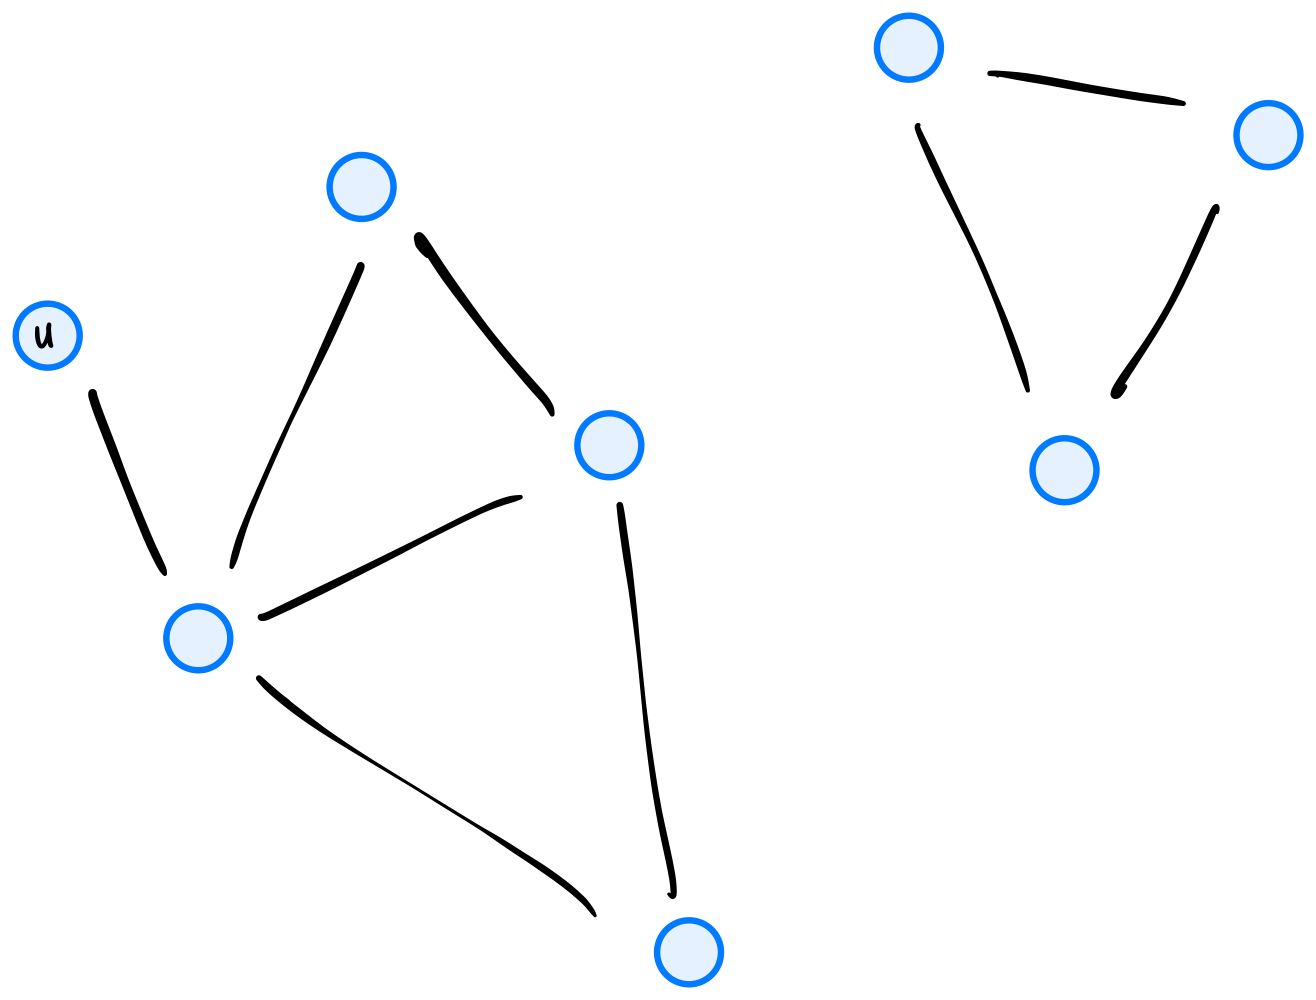
\includegraphics[width=.4\textwidth]{./g4.png}

\begin{soln}
    12
\end{soln}

\end{prob}
